\documentclass[tikz,border=5pt]{standalone}
\usepackage[utf8]{inputenc}
\usepackage[T1]{fontenc}
\usepackage{amsmath,amssymb}
\usepackage{lmodern}
\usetikzlibrary{arrows.meta}

\definecolor{boxbg}{HTML}{1d1d1f}
\definecolor{bluebg}{HTML}{142436}
\definecolor{amberbg}{HTML}{2c2214}
\definecolor{redbg}{HTML}{2e1517}
\definecolor{lighttext}{HTML}{f5f5f7}
\definecolor{subtext}{HTML}{d1d1d6}
\definecolor{muted}{HTML}{86868b}
\definecolor{amber}{HTML}{ff9f0a}
\definecolor{amberlight}{HTML}{ffd60a}
\definecolor{blueaccent}{HTML}{2997ff}
\definecolor{cyanlight}{HTML}{5ac8fa}
\definecolor{redaccent}{HTML}{ff453a}
\definecolor{redlight}{HTML}{ff6961}

\begin{document}
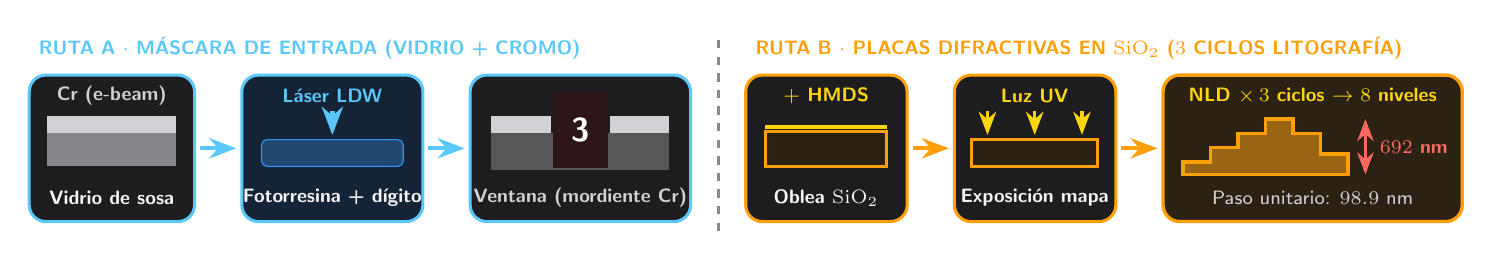
\begin{tikzpicture}[font=\sffamily,>=Stealth]

% ===================== RUTA A: MÁSCARA DE ENTRADA =====================
\node[anchor=west,text=cyanlight,font=\sffamily\bfseries\scriptsize] at (0.05,2.42)
  {RUTA A $\cdot$ MÁSCARA DE ENTRADA (VIDRIO + CROMO)};

% Paso A1
\draw[cyanlight,fill=boxbg,rounded corners=6pt,line width=1.1pt] (0.05,0.22) rectangle (2.15,2.08);
\node[text=subtext,font=\sffamily\scriptsize\bfseries] at (1.10,1.82) {Cr (\emph{e-beam})};
\fill[subtext] (0.28,1.34) rectangle (1.92,1.56);
\fill[muted]   (0.28,0.92) rectangle (1.92,1.34);
\node[text=lighttext,font=\sffamily\scriptsize\bfseries] at (1.10,0.52) {Vidrio de sosa};

\draw[->,cyanlight,line width=1.5pt] (2.22,1.15) -- (2.68,1.15);

% Paso A2
\draw[cyanlight,fill=bluebg,rounded corners=6pt,line width=1.1pt] (2.75,0.22) rectangle (5.05,2.08);
\node[text=cyanlight,font=\sffamily\scriptsize\bfseries] at (3.90,1.82) {Láser LDW};
\draw[->,cyanlight,line width=1.6pt] (3.90,1.62) -- (3.90,1.32);
\draw[blueaccent,fill=blueaccent!35!boxbg,rounded corners=2pt] (3.00,0.92) rectangle (4.80,1.26);
\node[text=lighttext,font=\sffamily\scriptsize\bfseries] at (3.90,0.52) {Fotorresina + dígito};

\draw[->,cyanlight,line width=1.5pt] (5.12,1.15) -- (5.58,1.15);

% Paso A3
\draw[cyanlight,fill=boxbg,rounded corners=6pt,line width=1.1pt] (5.65,0.22) rectangle (8.45,2.08);
\fill[muted!55!boxbg] (5.92,0.88) rectangle (8.18,1.34);
\fill[subtext] (5.92,1.34) rectangle (6.68,1.56);
\fill[subtext] (7.42,1.34) rectangle (8.18,1.56);
\fill[redbg]   (6.70,0.90) rectangle (7.40,1.86);
\node[text=white,font=\sffamily\bfseries\large] at (7.05,1.38) {3};
\node[text=subtext,font=\sffamily\scriptsize\bfseries] at (7.05,0.52) {Ventana (mordiente Cr)};

% Separador vertical
\draw[muted,dashed,line width=1.0pt] (8.80,0.10) -- (8.80,2.52);

% ===================== RUTA B: PLACAS DIFRACTIVAS =====================
\node[anchor=west,text=amber,font=\sffamily\bfseries\scriptsize] at (9.15,2.42)
  {RUTA B $\cdot$ PLACAS DIFRACTIVAS EN $\mathrm{SiO_2}$ ($3$ CICLOS LITOGRAFÍA)};

% Paso B1
\draw[amber,fill=boxbg,rounded corners=6pt,line width=1.1pt] (9.15,0.22) rectangle (11.20,2.08);
\node[text=amberlight,font=\sffamily\scriptsize\bfseries] at (10.17,1.82) {$+$ HMDS};
\draw[amberlight,line width=1.5pt] (9.40,1.42) -- (10.94,1.42);
\draw[amber,fill=amberbg,line width=1.0pt] (9.40,0.92) rectangle (10.94,1.36);
\node[text=lighttext,font=\sffamily\scriptsize\bfseries] at (10.17,0.52) {Oblea $\mathrm{SiO_2}$};

\draw[->,amber,line width=1.5pt] (11.27,1.15) -- (11.73,1.15);

% Paso B2
\draw[amber,fill=boxbg,rounded corners=6pt,line width=1.1pt] (11.80,0.22) rectangle (13.85,2.08);
\node[text=amberlight,font=\sffamily\scriptsize\bfseries] at (12.82,1.82) {Luz UV};
\draw[->,amberlight,line width=1.2pt] (12.22,1.62) -- (12.22,1.32);
\draw[->,amberlight,line width=1.2pt] (12.82,1.62) -- (12.82,1.32);
\draw[->,amberlight,line width=1.2pt] (13.42,1.62) -- (13.42,1.32);
\draw[amber,fill=amberbg,line width=1.0pt] (12.02,0.92) rectangle (13.62,1.26);
\node[text=lighttext,font=\sffamily\scriptsize\bfseries] at (12.82,0.52) {Exposición mapa};

\draw[->,amber,line width=1.5pt] (13.92,1.15) -- (14.38,1.15);

% Paso B3: Escalera 8 niveles
\draw[amber,fill=amberbg,rounded corners=6pt,line width=1.2pt] (14.45,0.22) rectangle (18.25,2.08);
\node[text=amberlight,font=\sffamily\scriptsize\bfseries] at (16.35,1.82) {NLD $\times\,3$ ciclos $\rightarrow 8$ niveles};
\filldraw[fill=amber!55!boxbg,draw=amber,line width=1.3pt]
  (14.70,0.82) -- (14.70,0.98) -- (15.05,0.98) -- (15.05,1.16) --
  (15.40,1.16) -- (15.40,1.34) -- (15.75,1.34) -- (15.75,1.52) --
  (16.10,1.52) -- (16.10,1.34) -- (16.45,1.34) -- (16.45,1.08) --
  (16.80,1.08) -- (16.80,0.82) -- cycle;
\draw[<->,redlight,line width=1.1pt] (17.02,0.82) -- (17.02,1.52);
\node[anchor=west,text=redlight,font=\sffamily\scriptsize\bfseries] at (17.08,1.17) {$692\text{ nm}$};
\node[text=subtext,font=\sffamily\scriptsize] at (16.35,0.52) {Paso unitario: $98.9\text{ nm}$};

\end{tikzpicture}
\end{document}
